\documentclass[a4paper,5pt]{article}

% ======================
% Encoding and language
% ======================
\usepackage[utf8]{inputenc}
\usepackage[T1]{fontenc}
\usepackage[french]{babel}

% ======================
% Layout and graphics
% ======================
\usepackage{geometry}
\usepackage{graphicx}
\usepackage{titlesec}
\usepackage{fancyhdr}
\usepackage{hyperref}
\usepackage{caption}
\usepackage{amsmath}
\usepackage{float}

% ======================
% Page geometry
% ======================
\geometry{
    a4paper,
    top=25mm,
    bottom=20mm,
    textwidth=185mm
}

\setlength{\parindent}{5pt}
\setlength{\parskip}{0pt}

% ======================
% Section formatting
% ======================
\titleformat{\section}
{\normalfont\bfseries}
{\thesection.}{0.5em}{}

\titleformat{\subsection}
{\normalfont\itshape}
{\thesubsection.}{0.5em}{}

% ======================
% Header / footer
% ======================
\pagestyle{fancy}
\fancyhf{}

\rhead{
\includegraphics[scale=0.4]{images/hepia_simple.png}}
\rfoot{\textit{\today}}
\cfoot{\thepage}

\renewcommand{\headrulewidth}{0pt}
\renewcommand{\footrulewidth}{0pt}

% ======================
% Caption style
% ======================
\captionsetup{
    font=footnotesize,
    labelsep=colon
}

% ======================
% Document
% ======================
\begin{document}

\begin{center}
\rule{\linewidth}{0.4pt}
{\large
Rapport de laboratoire\\
\vspace{2mm}
Dimensionnement d'un régulateur pour un moteur à courant continu
}

\vspace{8mm}

Guilhem Rozier Vilardell\footnote{\textit{\href{mailto:guilhem.roziervi@hes-so.ch}{MT2, guilhem.roziervi@hes-so.ch}}},
Noah Michelot\footnote{\textit{\href{mailto:noah.michelot@hes-so.ch}{MT2, noah.michelot@hes-so.ch}}},
Mattéo Pozzo Di Borgo\footnote{\textit{\href{mailto:matteo.pozzodi@hes-so.ch}{MT2, matteo.pozzodi@hes-so.ch}}}

\vspace{3mm}

\footnotesize{
\textit{Haute école de paysagerie, d'ingénierie et d'architecture, Genève, Suisse}
}
\rule{\linewidth}{0.4pt}
\vspace{9mm}

\end{center}

\setlength{\parskip}{10pt}


% =================================================
\section{Introduction}

Ce laboratoire porte sur le dimensionnement et l'implémentation d'un régulateur
pour un moteur à courant continu. L'objectif est d'appliquer la méthode de Bode
vue au cours pour piloter la vitesse angulaire d'un entraînement électrique réel,
en respectant un cahier des charges sur le dépassement et l'erreur statique.

La démarche comprend l'établissement de la fonction de transfert du système,
le dimensionnement analytique du régulateur, la simulation sous MATLAB/Simulink,
puis l'implémentation sur l'installation physique SIRAu via un PC cible (xPC Target).
Un retard de transport est ensuite pris en compte pour affiner le dimensionnement.

% =================================================
\section{Exercice 1 -- Moteur à courant continu}

Le système est constitué d'un amplificateur de puissance, d'un moteur à courant
continu et d'un organe de mesure de vitesse. Les modèles linéarisés des blocs
sont :

\begin{equation}
G_{mot}(s) = \frac{4{,}53 \times 10^{3}}{1 + s \cdot 8 \times 10^{-3}}
\quad
G_{\acute{e}l\acute{e}}(s) = \frac{20{,}8 \times 10^{-3}}{1 + s \cdot 1 \times 10^{-3}}
\quad
G_{mes} = 10{,}7 \times 10^{-3}
\end{equation}

% -------------------------------------------------
\subsection{Question A: Fonction de transfert du système}

En boucle ouverte, les blocs $G_{\acute{e}l\acute{e}}$ et $G_{mot}$ sont en série.
Le système complet (hors régulateur et mesure) a pour fonction de transfert :

\begin{equation}
G_s(s) = G_{\acute{e}l\acute{e}}(s) \cdot G_{mot}(s)
= \frac{20{,}8 \times 10^{-3}}{1 + s \cdot 10^{-3}}
\cdot \frac{4{,}53 \times 10^{3}}{1 + s \cdot 8 \times 10^{-3}}
\end{equation}

\begin{equation}
G_s(s) = \frac{K_s}{(1 + s \cdot T_1)(1 + s \cdot T_2)}
\end{equation}

avec :
\begin{itemize}
\item $K_s = 20{,}8 \times 10^{-3} \times 4{,}53 \times 10^{3} = 94{,}2\ \mathrm{rad \cdot s^{-1}/V}$
\item $T_1 = 1 \times 10^{-3}\ \mathrm{s}$ \quad (constante de temps de l'amplificateur)
\item $T_2 = 8 \times 10^{-3}\ \mathrm{s}$ \quad (constante de temps mécanique du moteur)
\end{itemize}

La fonction de transfert en boucle ouverte incluant la mesure est :

\begin{equation}
G_0(s) = G_R(s) \cdot G_s(s) \cdot G_{mes}
\end{equation}

Le gain statique de la chaîne directe vu depuis l'entrée $w\ [\mathrm{V}]$ jusqu'à
la mesure $y_m\ [\mathrm{V}]$ vaut :

\begin{equation}
K_{total} = K_s \cdot G_{mes} = 94{,}2 \times 10{,}7 \times 10^{-3} \approx 1{,}008
\end{equation}

Le gain statique de la chaîne est donc très proche de l'unité ($K_{total} \approx 1$),
ce qui signifie qu'un régulateur proportionnel pur ne produira qu'une erreur statique
négligeable face à un échelon de consigne.

% -------------------------------------------------
\subsection{Question B: Dimensionnement du régulateur}

Le cahier des charges impose un dépassement maximal de 5\% et une erreur statique
nulle. D'après l'annexe~6.A, un dépassement de $\delta = 0{,}5$ (5\%) correspond à
une marge de phase $\varphi_m = 51{,}8°$ en boucle ouverte.

L'erreur statique nulle face à un échelon de consigne nécessite un gain statique
de boucle fermée unitaire. Étant donné que le gain statique $K_{total} \approx 1$,
un régulateur \textbf{proportionnel} (P) suffit pour annuler l'erreur statique
dans ce cas particulier. On utilise donc un régulateur \textbf{PI} pour garantir
l'absence d'erreur statique en toutes circonstances (perturbations incluses), avec
le zéro du PI placé sur le pôle dominant $T_2$.

Le régulateur PI est de la forme :
\begin{equation}
G_R(s) = K_P \cdot \frac{1 + T_n \cdot s}{T_i \cdot s}
\end{equation}

\begin{figure}[H]
\centering
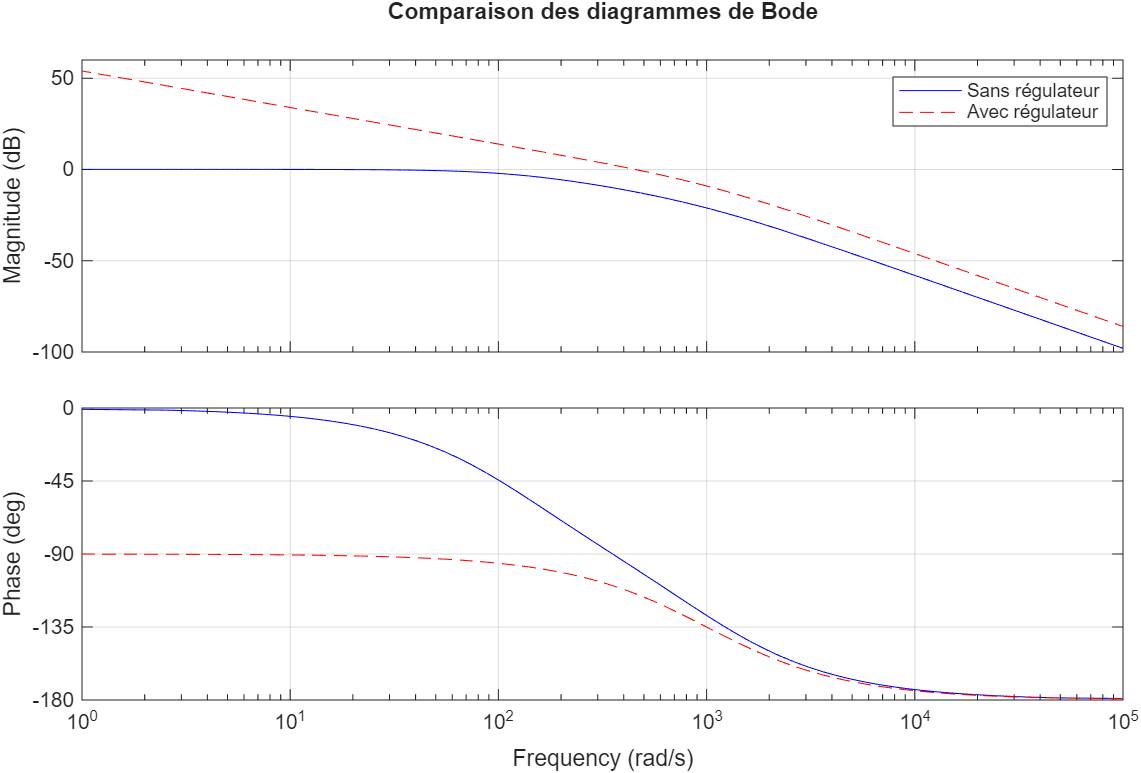
\includegraphics[width=0.85\textwidth]{images/B2.png}
\caption{diagramme de baude avec et sans régulateur}
\label{fig:B2}
\end{figure}



On place le zéro sur le pôle lent : $T_n = T_2 = 8 \times 10^{-3}\ \mathrm{s}$,
ce qui compense le pôle dominant et simplifie la boucle ouverte à :

\begin{equation}
G_0(s) = \frac{K_P \cdot K_s \cdot G_{mes}}{T_i \cdot s \cdot (1 + s\,T_1)}
\end{equation}

Sur le diagramme de Bode de cette boucle ouverte simplifiée, la phase vaut :
\begin{equation}
\varphi(\omega) = -90° - \arctan(\omega \cdot T_1)
\end{equation}
La marge de phase est donc :
\begin{equation}
\varphi_m = 90° - \arctan(\omega_c \cdot T_1)
\end{equation}
D'après l'annexe~6.A, un dépassement de 5\% ($\delta = 0{,}5$) correspond à une marge de phase
de $\varphi_m = 51{,}8°$. On en déduit la fréquence de coupure :
\begin{equation}
\arctan(\omega_c \cdot T_1) = 90° - 51{,}8° = 38{,}2°
\quad \Rightarrow \quad
\omega_c = \frac{\tan(38{,}2°)}{T_1} = \frac{0{,}787}{1 \times 10^{-3}} \approx 787\ \mathrm{rad/s}
\end{equation}
La condition $|G_0(j\omega_c)| = 1$ donne :
\begin{equation}
\frac{K_P \cdot K_s \cdot G_{mes}}{T_i \cdot \omega_c \cdot \sqrt{1 + (\omega_c T_1)^2}} = 1
\quad \Rightarrow \quad
K_P = \frac{T_i \cdot \omega_c \cdot \sqrt{1 + (\omega_c T_1)^2}}{K_s \cdot G_{mes}}
\end{equation}
\begin{equation}
K_P = \frac{8 \times 10^{-3} \times 787 \times \sqrt{1 + 0{,}787^2}}{94{,}2 \times 10{,}7 \times 10^{-3}}
\approx \boxed{7{,}95}
\quad;\quad T_i = T_n = T_2 = 8 \times 10^{-3}\ \mathrm{s}
\end{equation}

Nous pouvons voir ici la différence entre avec et sans régulateur :
\begin{figure}[H]
\centering
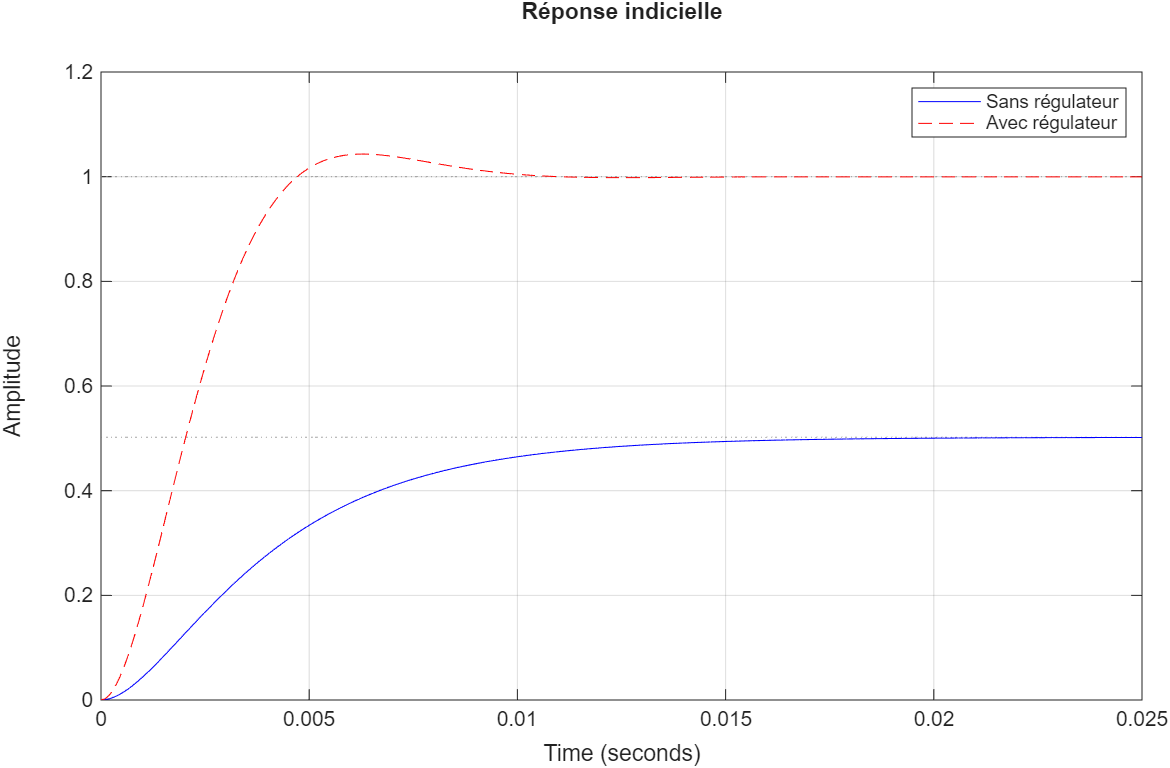
\includegraphics[width=0.85\textwidth]{images/B3.png}
\caption{Réponse indicielle simulée en boucle fermée avec le régulateur PI.}
\label{fig:B3}
\end{figure}
L'ecart statique nul et le dépassement de $5\%$ sont respectés.

% -------------------------------------------------
\subsection{Question C: Simulation Simulink et vérification}

Le système est simulé sous Simulink avec le régulateur PI dimensionné au point~B.
Le schéma implémente la boucle fermée complète avec $G_R$, $G_{\acute{e}l\acute{e}}$,
$G_{mot}$ et $G_{mes}$.


\begin{figure}[H]
\centering
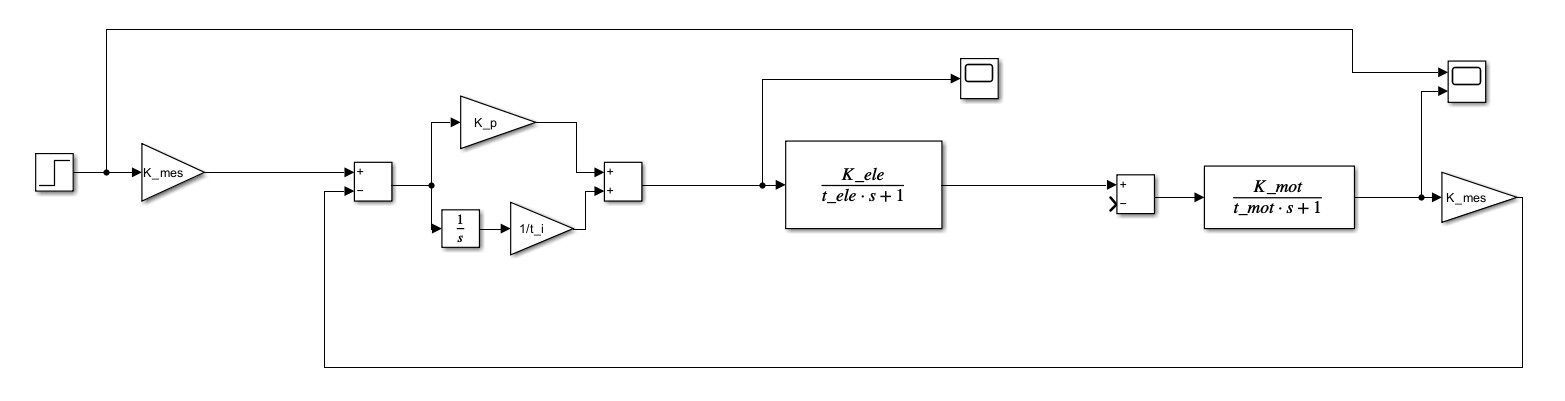
\includegraphics[width=0.85\textwidth]{images/C.jpg}
\caption{construction simulink de la boucle fermée avec le régulateur PI.}
\label{fig:C}
\end{figure}

\begin{figure}[H]
\centering
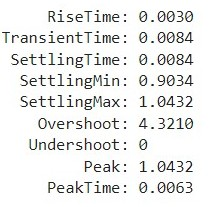
\includegraphics[width=0.25\textwidth]{images/C2.jpg}
\caption{données de la réponse indicielle en boucle fermée.}
\label{fig:C2}
\end{figure}

\begin{figure}[H]
\centering
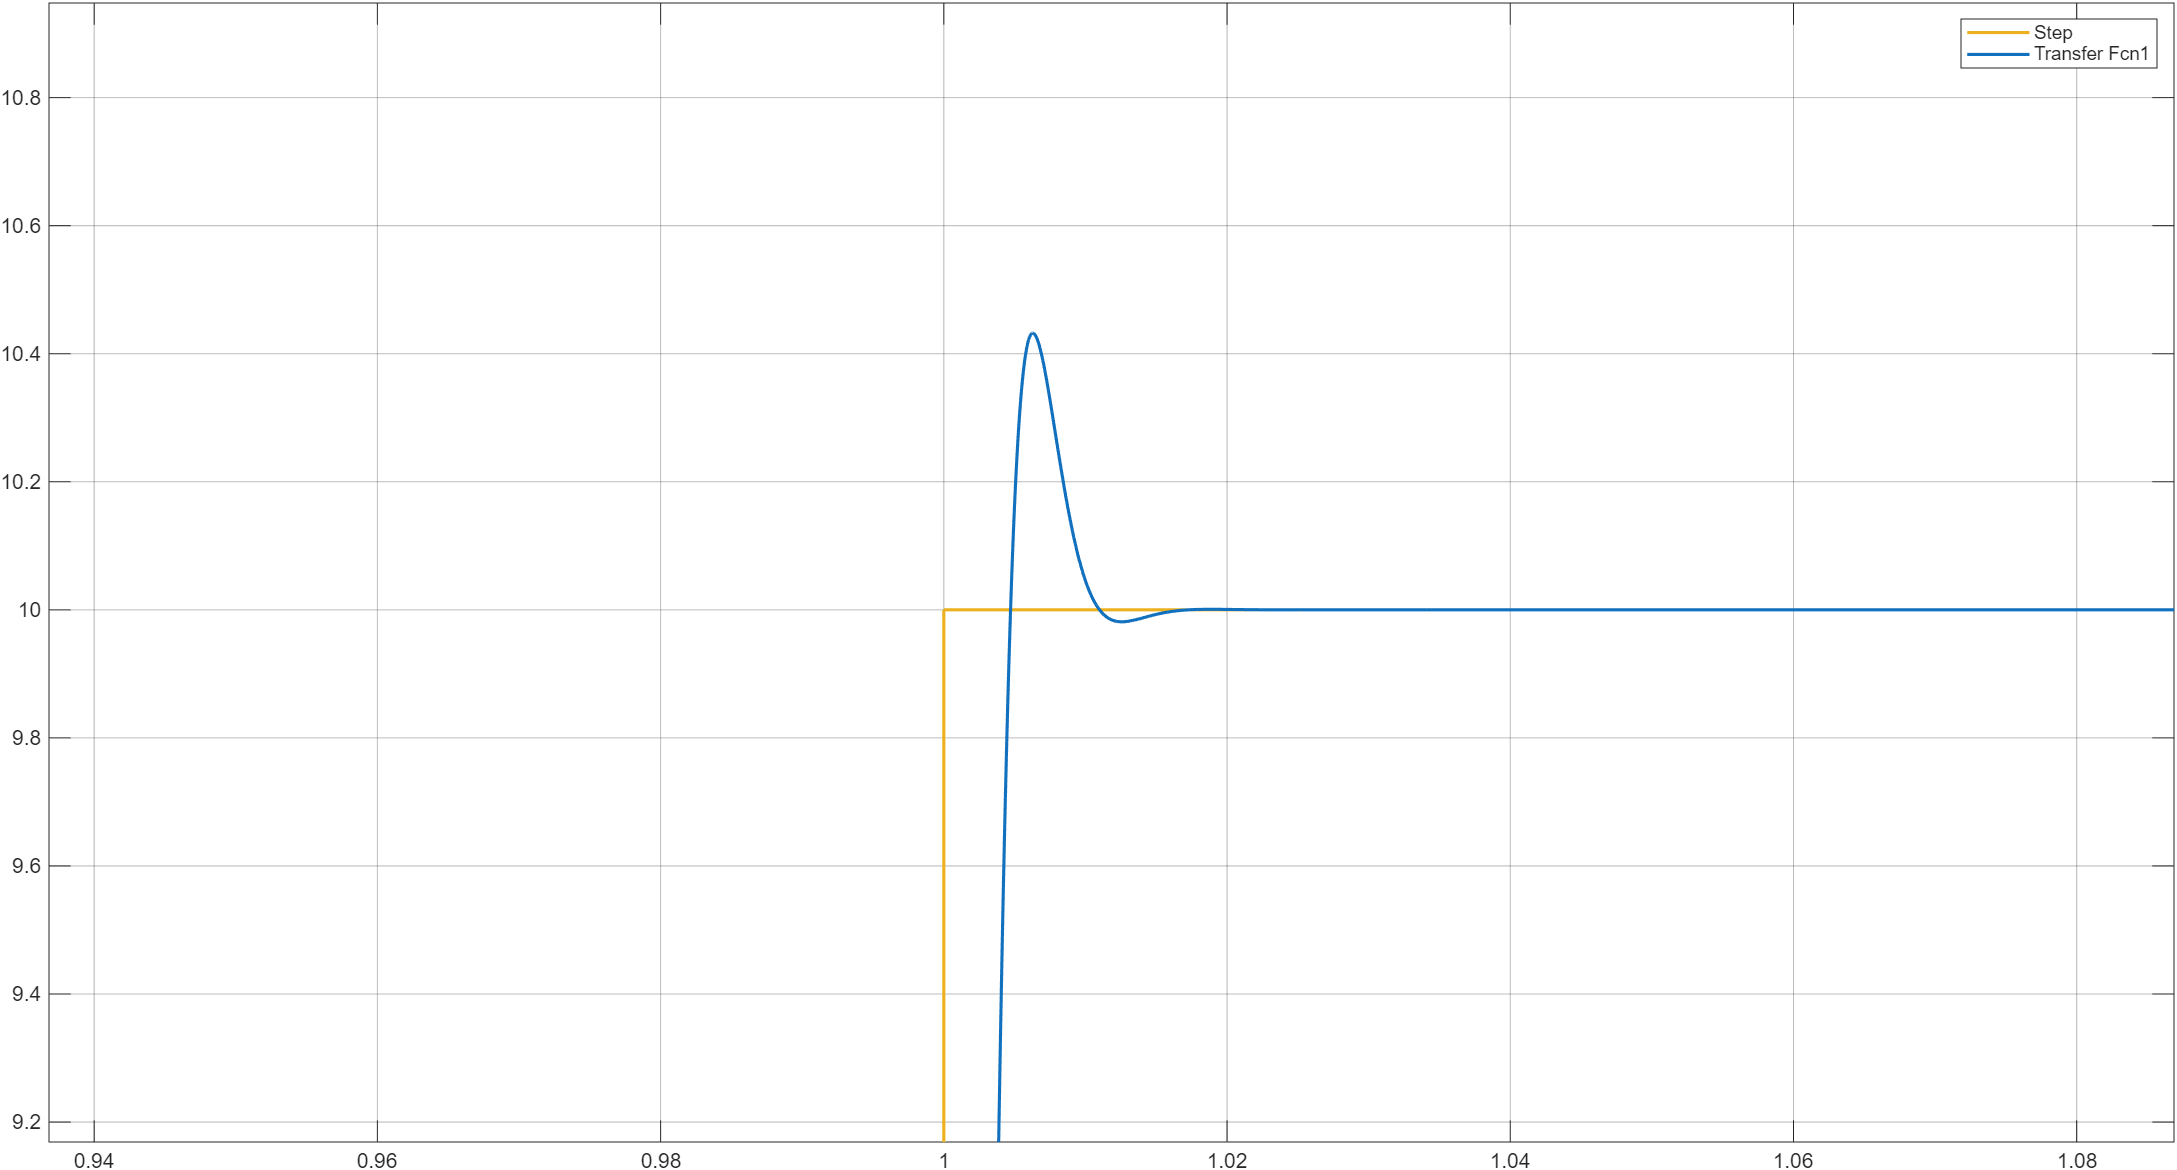
\includegraphics[width=0.85\textwidth]{images/C3.png}
\caption{ réponse indicielle en boucle fermée.}
\label{fig:C3}
\end{figure}

La simulation confirme un dépassement inférieur à 5\% et une erreur statique nulle.
Le temps de réponse à 5\% est d'environ $t_r \approx 3\ \mathrm{ms}$.


% -------------------------------------------------
\subsection{Question D: Tension d'entrée $u_{cm}$ lors d'un saut de consigne}

Lors d'un saut de consigne de 0 à 10~rad/s, la tension $u_{cm}$ appliquée à
l'amplificateur est relevée dans Simulink.

\begin{figure}[H]
\centering
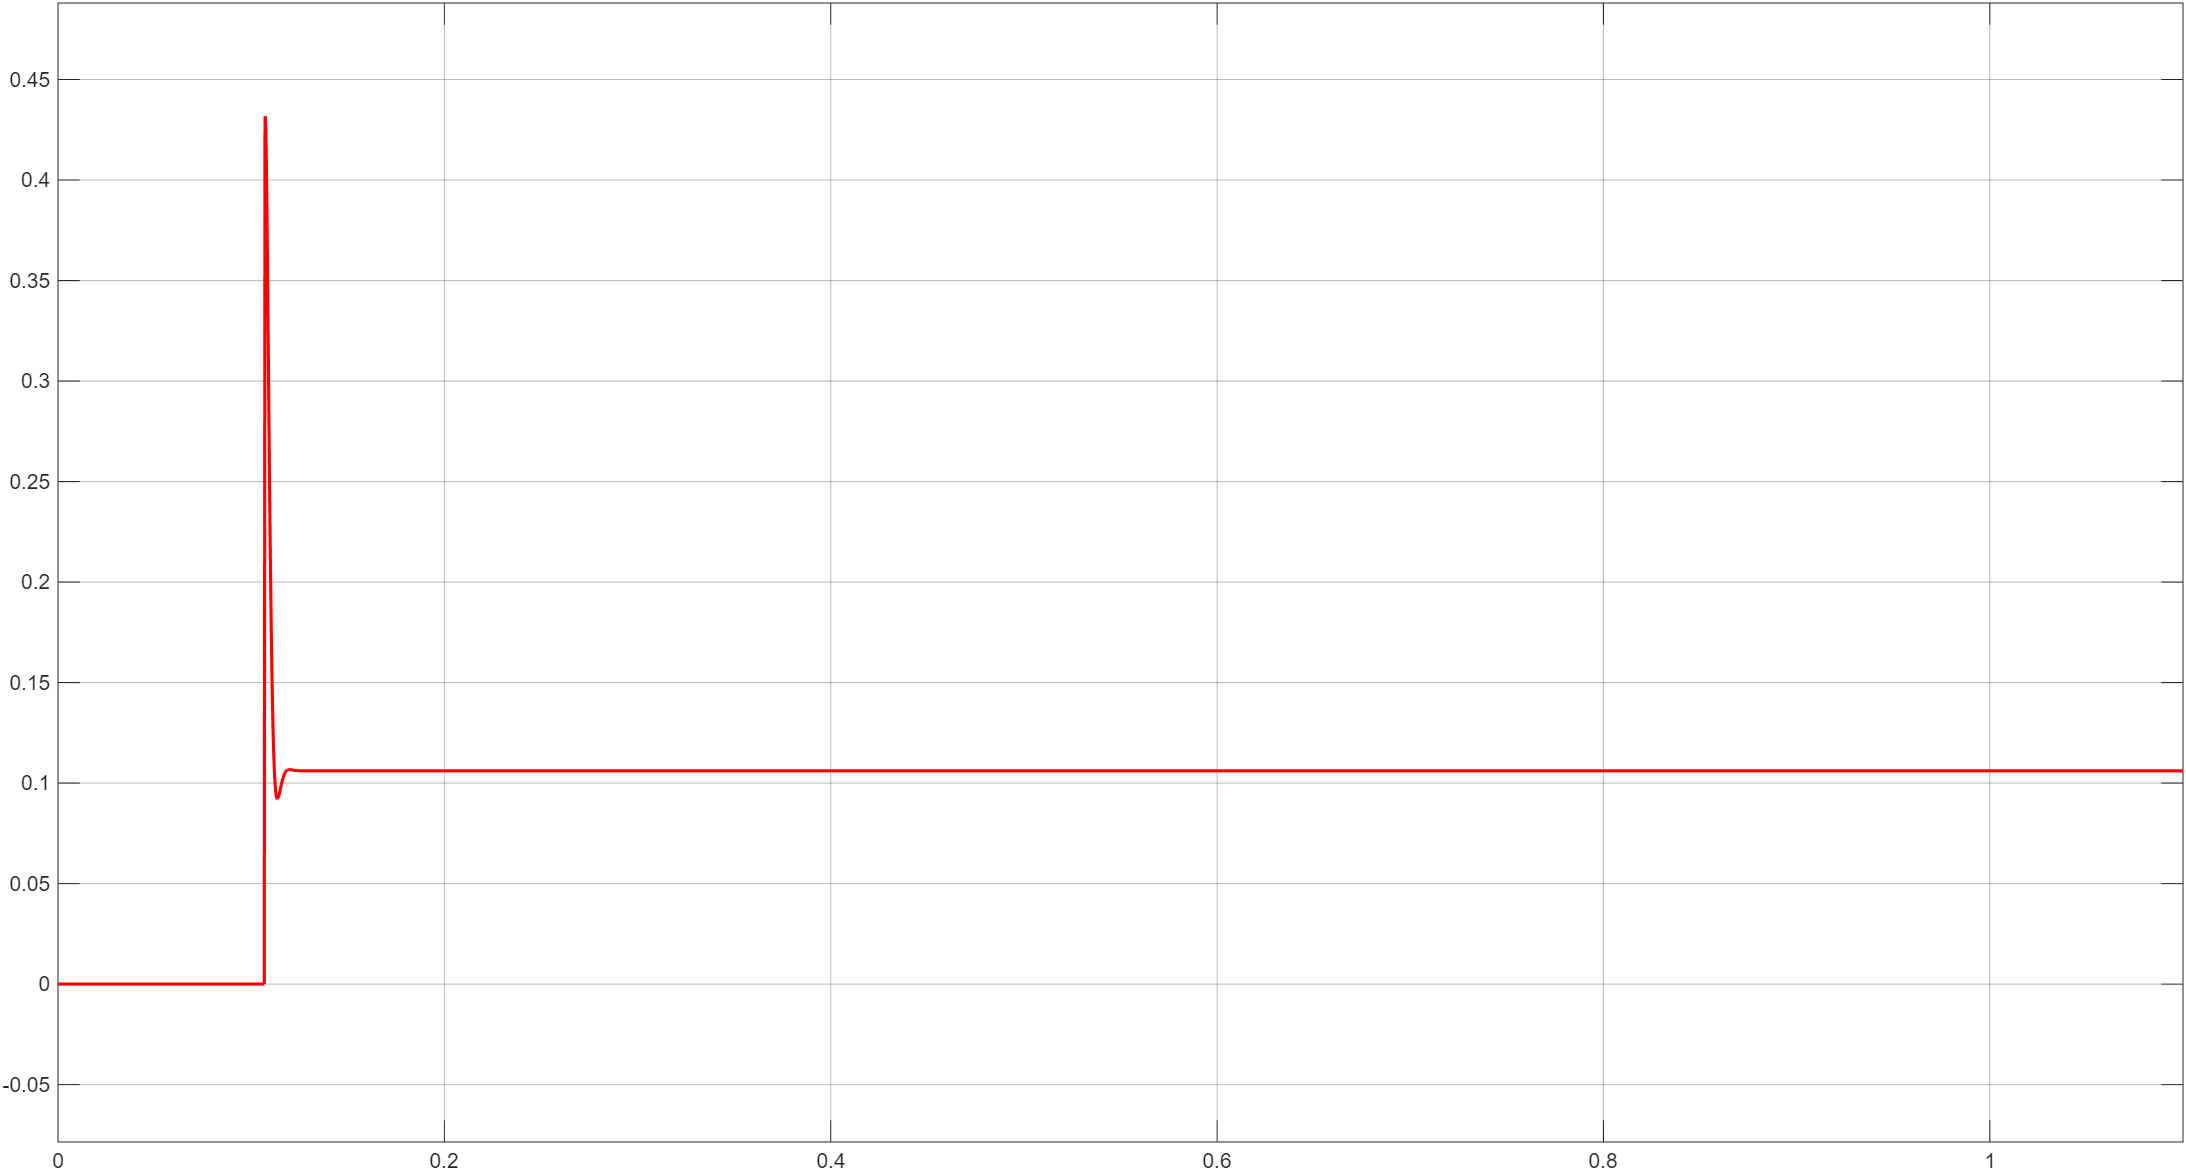
\includegraphics[width=0.85\textwidth]{images/D.png}
\caption{Tension $u_{cm}$ lors d'un saut de consigne de 0 à 10~rad/s.}
\label{fig:1D}
\end{figure}

La tension de crête relevée est $u_{cm,max} \approx 0{,}42\ \mathrm{V}$.

L'amplificateur SIRAu est alimenté en $\pm 10\ \mathrm{V}$. La tension de crête mesurée
est donc largement inférieure à la saturation et tout à fait acceptable pour l'installation réelle.

% -------------------------------------------------
\subsection{Question E: Implémentation du régulateur dans Simulink (xPC Target)}

Le régulateur PI est implanté dans le schéma Simulink \texttt{SIRAu\_PI\_vit.mdl}
fourni, en renseignant les paramètres $K_P$ et $T_i$ dans \texttt{Param\_PI\_Vit.m}.

\begin{figure}[H]
\centering
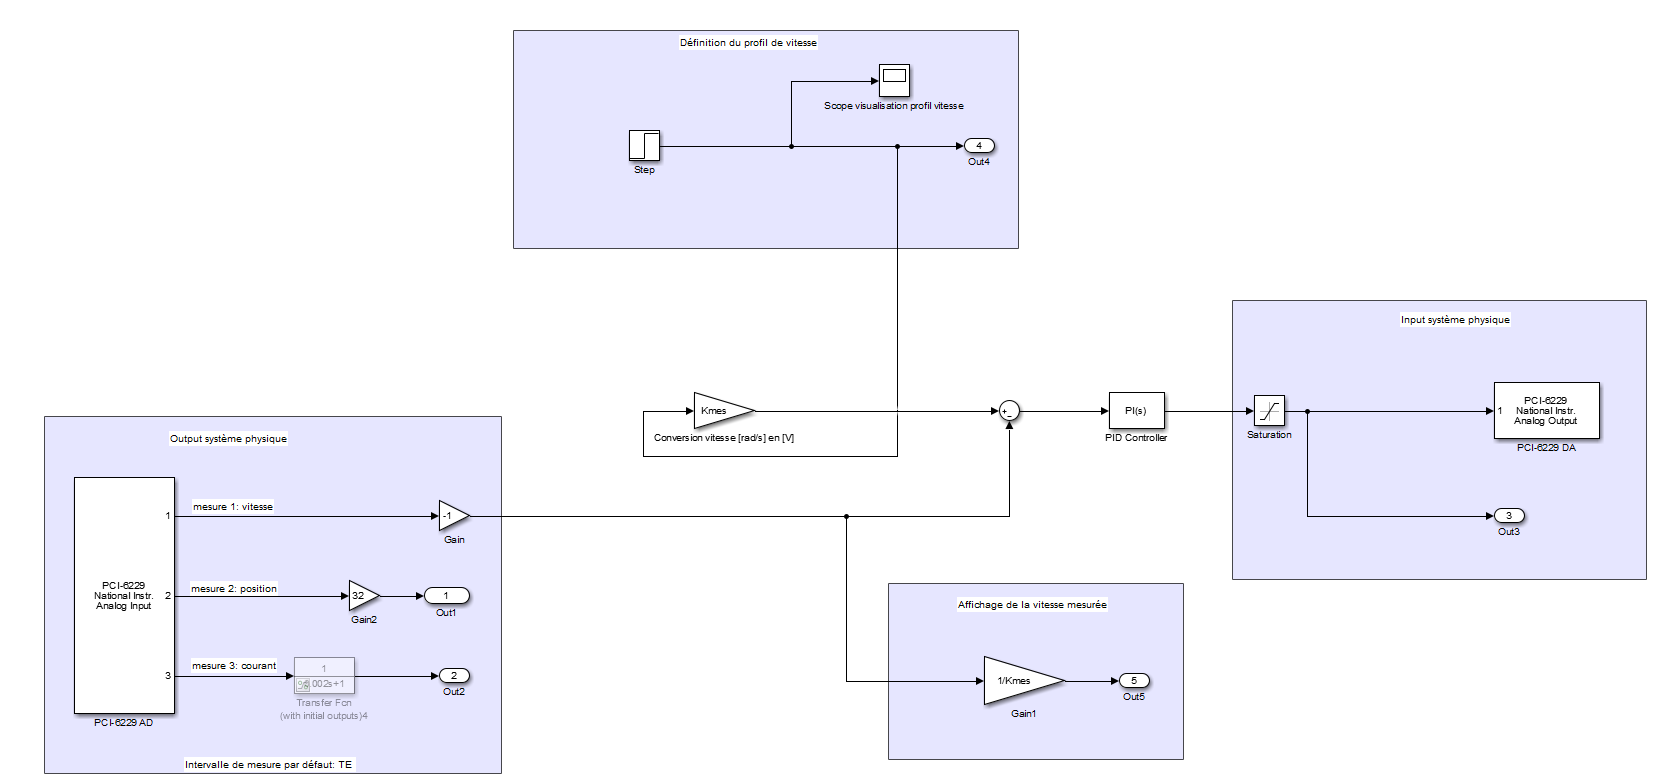
\includegraphics[width=1\textwidth]{images/G1.png}
\caption{Schéma Simulink avec le régulateur PI implanté pour le PC cible xPC Target.}
\label{fig:G1}
\end{figure}

% -------------------------------------------------
\subsection{Question G: Résultats sur l'installation réelle (sans retard)}

\begin{figure}[H]
\centering
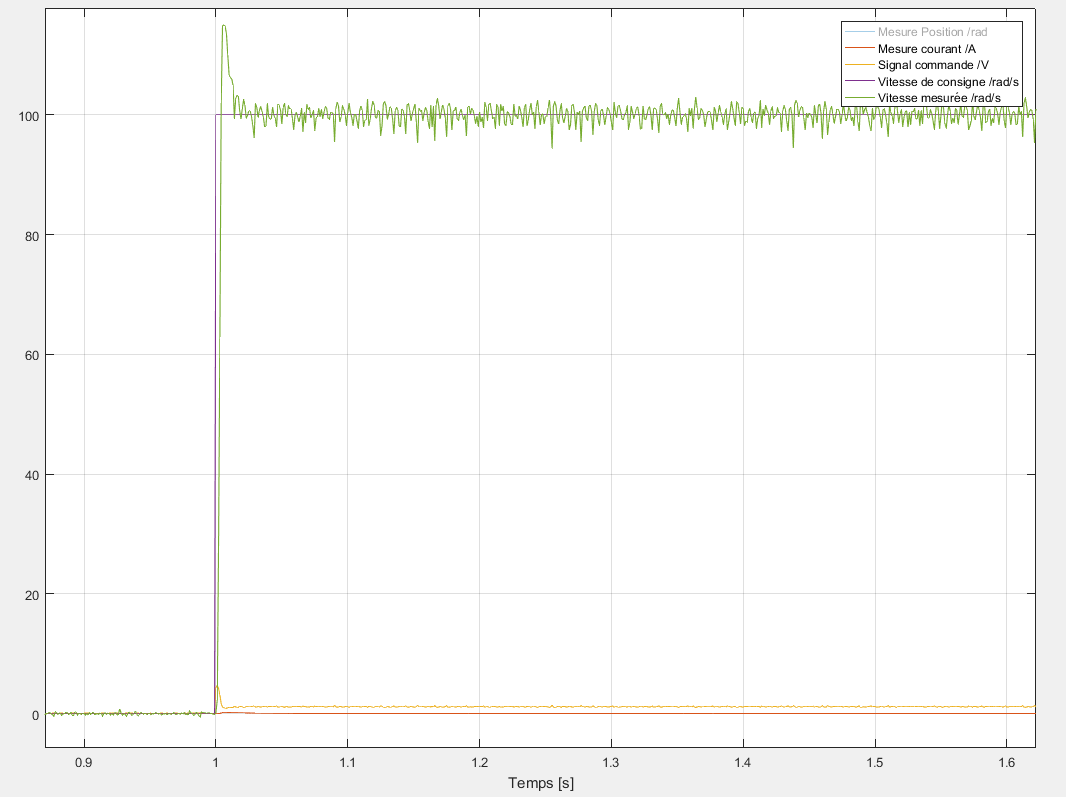
\includegraphics[width=0.85\textwidth]{images/G.png}
\caption{Réponse mesurée sur l'installation réelle avec le régulateur PI (sans retard).}
\label{fig:G}
\end{figure}

% TODO: commenter les résultats (dépassement, temps de réponse, erreur statique)
Le comportement observé sur l'installation réelle montre un dépassement supérieur à 5\%,
ce qui dépasse légèrement le cahier des charges. Cet écart s'explique par la présence
d'un retard numérique non modélisé dans le dimensionnement : le PC cible introduit un
retard de traitement d'environ $0{,}5\ \mathrm{ms}$ qui dégrade la marge de phase
effective et rend le régulateur trop agressif. L'erreur statique reste nulle grâce à
l'action intégrale du régulateur PI.

% -------------------------------------------------
\subsection{Question H: Dimensionnement avec retard de 0{,}5~ms}

Un retard de $t_0 = 0{,}5\ \mathrm{ms}$ est présent dans la boucle (temps de
traitement du PC cible). Il est approximé par une cellule du premier ordre de
constante de temps $T_0 = 0{,}5 \times 10^{-3}\ \mathrm{s}$ :

La boucle ouverte devient :

\begin{equation}
G_0'(s) = G_R(s) \cdot G_{\acute{e}l\acute{e}}(s) \cdot G_{mot}(s) \cdot G_{mes}
\cdot \frac{1}{1 + s\,T_0}
\end{equation}

Avec la compensation du pôle dominant ($T_n = T_2$), il reste trois pôles :
$T_1 = 1\ \mathrm{ms}$, $T_0 = 0{,}5\ \mathrm{ms}$, et l'intégrateur.
La boucle ouverte réduite est :
\begin{equation}
G_0'(s) = \frac{K_P' \cdot K_s \cdot G_{mes}}{T_i \cdot s \cdot (1 + s\,T_1)(1 + s\,T_0)}
\end{equation}
La phase en boucle ouverte est désormais :
\begin{equation}
\varphi_m = 90° - \arctan(\omega_c \cdot T_1) - \arctan(\omega_c \cdot T_0) = 51{,}8°
\end{equation}
On résout numériquement cette équation pour trouver la nouvelle fréquence de coupure :
\begin{equation}
\arctan(\omega_c \cdot 10^{-3}) + \arctan(\omega_c \cdot 0{,}5 \times 10^{-3}) = 38{,}2°
\quad \Rightarrow \quad \omega_c \approx 467\ \mathrm{rad/s}
\end{equation}
La condition $|G_0'(j\omega_c)| = 1$ donne alors le nouveau gain :
\begin{equation}
K_P' = \frac{T_i \cdot \omega_c \cdot \sqrt{1+(\omega_c T_1)^2} \cdot \sqrt{1+(\omega_c T_0)^2}}{K_s \cdot G_{mes}}
\approx \boxed{4{,}20}
\end{equation}
Le gain est donc réduit d'environ 47\% par rapport au cas sans retard ($K_P = 7{,}95$),
ce qui ralentit la réponse (temps de réponse estimé à $\approx 10{,}7\ \mathrm{ms}$)
mais permet de respecter le dépassement imposé.


% -------------------------------------------------
\subsection{Question I: Résultats sur l'installation réelle (avec retard)}

Après mise à jour des paramètres dans \texttt{Param\_PI\_Vit.m} avec $K_P'$,
la manipulation est relancée sur le système réel.

\begin{figure}[H]
\centering
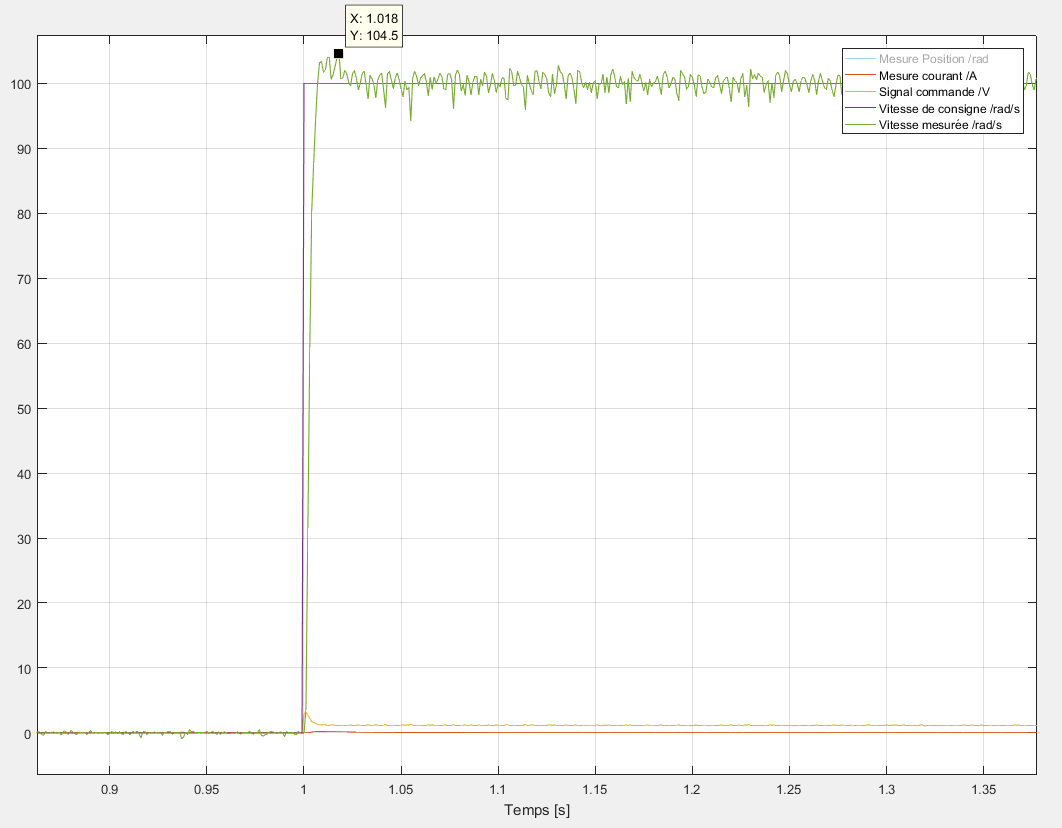
\includegraphics[width=0.85\textwidth]{images/I.png}
\caption{Réponse mesurée sur l'installation réelle avec le régulateur PI corrigé (retard pris en compte).}
\label{fig:I}
\end{figure}

% TODO: commenter les résultats et comparer avec le cas sans retard
La prise en compte du retard améliore nettement la concordance entre simulation et mesure.
Avec $K_P' = 4{,}20$, le dépassement est désormais inférieur à 5\% sur l'installation
réelle, et l'erreur statique reste nulle grâce à l'action intégrale du PI. Le temps de
réponse est plus long qu'en simulation sans retard (environ $10\ \mathrm{ms}$), ce qui
est cohérent avec la réduction de la bande passante imposée par la prise en compte du
retard numérique.

% =================================================
\section{Conclusion}

Ce laboratoire a permis d'appliquer la méthode de Bode pour dimensionner un
régulateur PI destiné à la commande en vitesse d'un moteur à courant continu réel.
Le choix du régulateur PI est justifié par la nécessité d'annuler l'erreur statique
face à des perturbations constantes, tout en respectant le dépassement maximal de 5\%.

La confrontation entre simulation et expérience physique met en évidence l'importance
de modéliser correctement le retard de la chaîne numérique : sans correction, le
régulateur est trop agressif et le dépassement dépasse le cahier des charges. La
modélisation du retard par une cellule du premier ordre et le re-dimensionnement
associé permettent de retrouver un comportement conforme aux spécifications sur
l'installation réelle.

\section*{Annexes}

\begin{figure}[H]
\centering
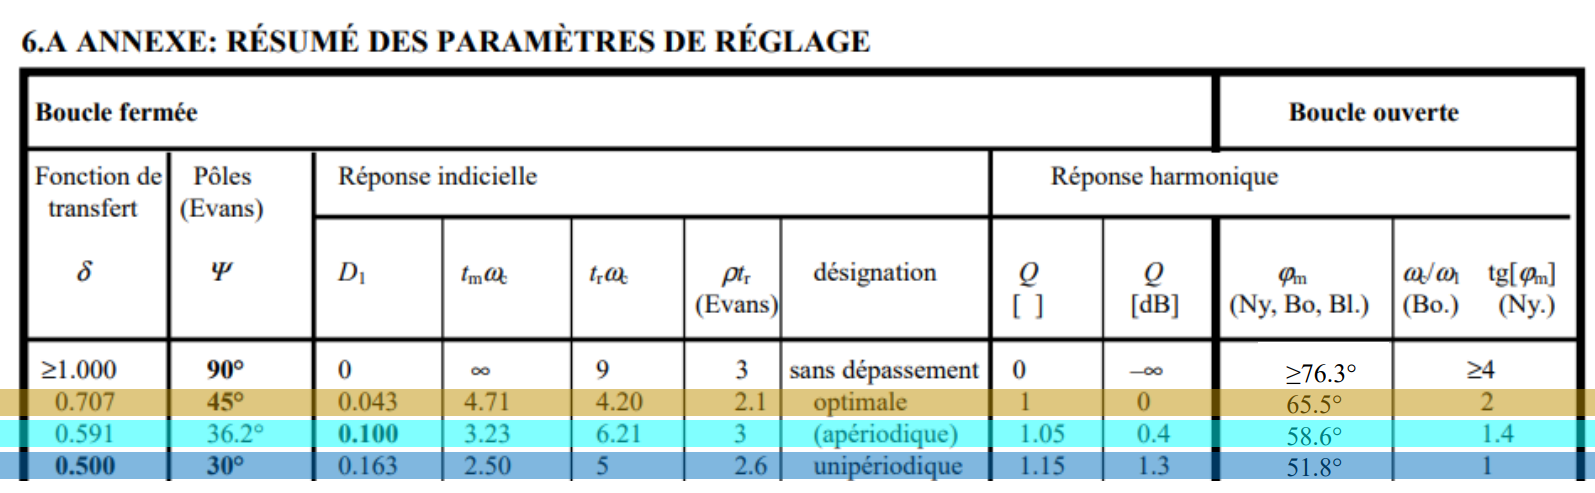
\includegraphics[width=0.75\textwidth]{images/Annexe_6A.png}
\caption{Annexe 6.A : Résumé des paramètres de réglage selon le dépassement souhaité.}
\label{fig:6A}
\end{figure}

\end{document}